\documentclass{report}

\usepackage{ugentstyle}
\begin{document}
	\maketitle{Beveiliging van netwerken en computers}
	\tableofcontents
	
	\chapter{Routing + DNS}
	De bedoeling van dit labo is een netwerkconfiguratie op te stellen en een DNS-server op te zetten die je in latere labo's nog zal gebruiken. Zorg er dus voor dat je de configuratie waar mogelijk persistent maakt, en eventueel de nodige commando's in scripts opneemt zodat je tijdens volgende labo's de opstelling snel kan herstellen.  Vooraleer aan de instellingen van de (fysieke) labotoestellen iets te veranderen maak je een volledige backup van de \textbackslash etc directory (tar -cvjf \textbackslash root \textbackslash backup\_etc.tar.bz2 \textbackslash etc).
	Editeer geen enkel configuratiebestand zonder er eerst een kopie van te maken!
	
	Voor dit labo werken we met groepjes van twee studenten. Iedere groep zal zich ontfermen over één DNS-domein dat vier hosts omvat (twee fysieke toestellen en twee virtuele machines). Ieder fysiek toestel zal dus als host fungeren voor één virtuele machine. Figuur \ref{fig:opstelling} geeft een algemeen overzicht van de opstelling voor één groep.
	\begin{figure}
		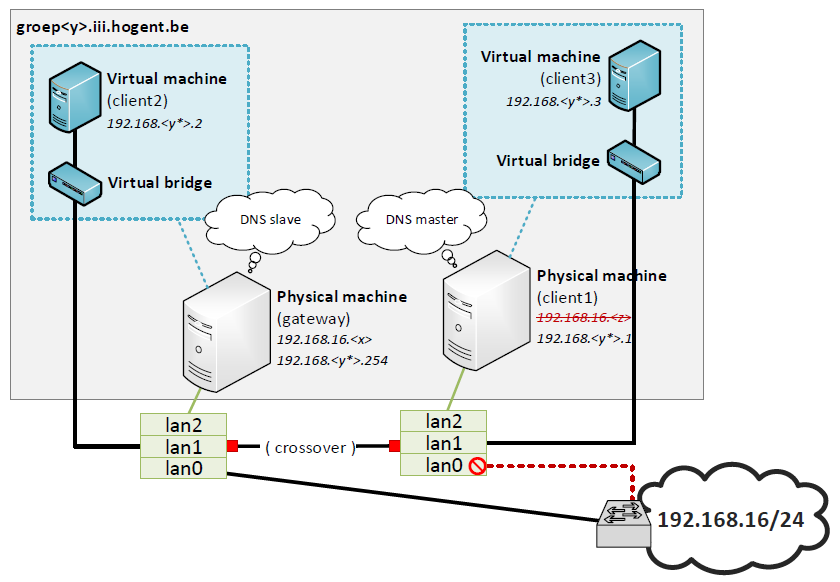
\includegraphics[width=\textwidth]{opstelling}
		\caption{Opstelling}
		\label{fig:opstelling}
	\end{figure}
	Voor de uitwerking van dit labo wordt de groep op figuur \ref{fig:groep} gebruikt.
	\begin{figure}
		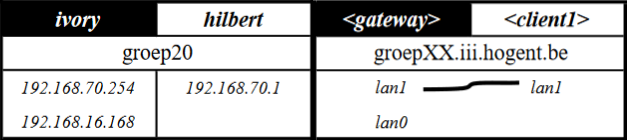
\includegraphics[width=\textwidth]{groep}
		\caption{Een groep}
		\label{fig:groep}
	\end{figure}
\section{Routing}
 Voor elke groep bestaat de opstelling uit vier verschillende hosts:
\begin{itemize}
	\item \textbf{gateway}: deze verbindt het interne netwerk van jouw groep met het HoGent netwerk via onze gateway 192.168.16.8. Dit toestel is via een crosskabel (lan1) verbonden met de tweede fysieke machine (client1).
	\item \textbf{client1}: deze is via een crosskabel (lan1) verbonden met de gateway. Merk op dat dit toestel niet rechtstreeks verbonden is met het HoGent netwerk!
	\item \textbf{client2}: dit is een virtuele machine die draait op de gateway. Deze virtuele machine is via een virtuele bridge verbonden met het interne netwerk (lan1) van de gateway.
	\item \textbf{client3}: dit is een virtuele machine die draait op client1. Deze virtuele machine is via een virtuele bridge verbonden met het interne netwerk (lan1) van client1.
	
\end{itemize}
\subsection{Configuratie IP-adressen}
Voor de netwerkconfiguratie maak je overal gebruik van statische IP-adressen (ook voor lan0 op de gateway). Om te testen kan je eerst gebruikmaken van het \textit{ip} commando, maar uiteindelijk is het eenvoudigst om een configuratiebestand te voorzien per interface. De configuratiebestanden vind je bij Fedora terug in de folder \texttt{/etc/sysconfig/network-scripts/}. 
\begin{itemize}
	\item \textbf{Gateway}: \begin{itemize}
								\item \texttt{ifcfg-lan0}:
									  		\begin{lstlisting}
DEVICE=lan0
BOOTPROTO=none
ONBOOT=yes
NETMASK=255.255.255.0
IPADDR=192.168.16.168
GATEWAY=192.168.16.8
											\end{lstlisting}
								\item \texttt{ifcfg-lan1}:
\begin{lstlisting}
DEVICE=lan0
BOOTPROTO=none
ONBOOT=yes
NETMASK=255.255.255.0
IPADDR=192.168.70.254
\end{lstlisting}											
							\end{itemize}
	\item \textbf{Client1}: 
	\begin{itemize}
		\item \texttt{ifcfg-lan1}:
		\begin{lstlisting}
DEVICE=lan1
BOOTPROTO=none
ONBOOT=yes
NETMASK=255.255.255.0
IPADDR=192.168.70.1
GATEWAY=192.168.70.254
		\end{lstlisting}										
	\end{itemize}

	\item \textbf{Client2}: 
\begin{itemize}
	\item \texttt{ifcfg-enp0s3}:
	\begin{lstlisting}
DEVICE=enp0s3
BOOTPROTO=none
ONBOOT=yes
NETMASK=255.255.255.0
IPADDR=192.168.70.2
GATEWAY=192.168.70.254
	\end{lstlisting}										
\end{itemize}

	\item \textbf{Client3}: 
\begin{itemize}
	\item \texttt{ifcfg-enp0s3}:
	\begin{lstlisting}
DEVICE=enp0s3
BOOTPROTO=none
ONBOOT=yes
NETMASK=255.255.255.0
IPADDR=192.168.70.3
GATEWAY=192.168.70.254
	\end{lstlisting}										
\end{itemize}

\end{itemize}

\subsection{OSPF}

Op de gateway gebruik je OSPF om de route naar jouw subnet te multicasten. Als router-software maak je gebruik van quagga en twee zelfgemaakte configuratiebestanden zebra.conf en ospfd.conf die je in de directory \texttt{/etc/quagga} plaatst. Aangezien iedere gateway rechtstreeks verbonden is met het 192.168.16.0/24 netwerk laten we dit overeenstemmen met area 0. Het is dus niet nodig om bijkomende areas in het leven te roepen!
Ken aan je interfaces geen IP-adressen toe via quagga maar doe dit dus op de traditionele manier met het commando ip of via ifcfg-files.
Vergeet niet om routing actief te zetten op de nodige hosts.
Om te testen of je configuratie werkt, moet je zowel de zebra daemon als de ospfd daemon starten. 

\begin{itemize}
	\item \textbf{zebra.conf}:
		\begin{lstlisting}
hostname ivory
password pass
enable password pass
log stdout
!
interface lan0
!
interface lan1
!
		\end{lstlisting}
	\item \textbf{ospfd.conf}:
		\begin{lstlisting}
hostname ivory
password pass
enable password pass
log stdout
!
interface lan0
!
interface lan1
!
router ospf
	redistribute connected
	network 192.168.16.0/24 area 0.0.0.0
!
\end{lstlisting}

\end{itemize}
Voeg \texttt{net.ipv4.ip\_forward = 1} toe aan het bestand \texttt{/etc/sysctl.conf}. 
Voer nu het commando \texttt{systemctl status/restart/enable zebra/ospfd} uit. \textit{Restart} zal de daemon herstarten en \textit{enable} geeft aan dat de daemon bij de bootprocedure moet opgestart worden. Met \textit{status} kan nagegaan worden of dat de configuratie correct verlopen is.
\section{DNS}
Binnen de opstelling configureer je ook twee DNS-servers die verantwoordelijk zijn voor het subdomein van de groep (groep20.iii.hogent.be). \textbf{client1} doet dienst als primaire (master) DNS-server, de \textbf{gateway} als secundaire (slave) DNS-server. Binnen je domein voorzie je zowel een forward als een reverse DNS lookup zone. Alle aanvragen die niet voor jouw domein bedoeld zijn stuur je via een \textbf{forwarder} door naar 192.168.16.8. 
\subsection{Configuratie named}
 Wij hebben reeds voor jou een DNS-root-server geconfigureerd. Bijgevolg kunnen alle DNS-aanvragen die geen betrekking hebben op jouw domein doorgestuurd worden naar 192.168.16.8. Dit is ook de default-gateway van de router en moet als dusdanig worden ingesteld. Jouw DNS-server voorziet in de naamgeving voor de vier hosts in het domein. Om voldoende redundantie te hebben, configureer je op de gateway een secundaire nameserver.

Voor DNS maken we gebruik van de BIND/named service die reeds op de fysieke toestellen geïnstalleerd is. De configuratie moet je zelf nog aanpassen of aanmaken. Maak hiervoor gebruik van volgende directories en bestanden:

\begin{itemize}
	\item \texttt{/etc/named.conf}: algemene configuratie BIND/named.
	\item \texttt{/var/named/}: zonebestanden voor jouw domein
\end{itemize}


Om te testen of het configuratiebestand en de zonebestanden correct zijn, kan je respectievelijk gebruikmaken van de \texttt{named-checkconf} en \texttt{named-checkzone} commando's. Eenmaal de configuratie correct is, kan je de named service (her)starten via het systemctl commando.
Voor de virtuele machines gebruik je als hostname de naam van je toestel, gevolgd door 'VM'. De virtuele machine op computer Kronecker zal bv. de naam KroneckerVM hebben.
Voorzie zowel een forward als een reverse DNS lookup zone die de vier hosts bevat en test grondig uit! Aangezien veel services die we tijdens de labo's gebruiken steunen op reverse DNS, is het belangrijk dat deze correct geconfigureerd is. 
\begin{itemize}
	\item \textbf{/etc/named.conf}: 
	\begin{itemize}
		\item client1:
			\begin{lstlisting}
options {
	directory	"/var/named";
	dump-file	"/var/named/data/cache_dump.db";
	statistics-file	"/var/named/data/named_stats.txt";
	memstatistics-file "var/named/data/named_mem_stats.txt";
	allow-query	{ any; };
	recursion yes,
	empty-zones-enable no;
	forwarders { 192.168.16.8; };
};

logging {
	channel default_debug {
		syslog daemon;
		severity dynamic;
	}
};

zone "groep20.iii.hogent.be" IN {
	type master;
	file "groep20.iii.hogent.be";
	allow-transfer { 192.168.70.254; };
};

zone "70.168.192.in-addr.arpa" {
	type master;
	file "70.168.192.in-addr.arpa";
	allow-transfer { 192.168.70.254; };	
};

			\end{lstlisting}
		\item gateway: 
		\begin{lstlisting}
options {
	directory	"/var/named";
	dump-file	"/var/named/data/cache_dump.db";
	statistics-file	"/var/named/data/named_stats.txt";
	memstatistics-file "var/named/data/named_mem_stats.txt";
	allow-query	{ any; };
	recursion yes,
	empty-zones-enable no;
	forwarders { 192.168.16.8; };
};

logging {
	channel default_debug {
		syslog daemon;
		severity dynamic;
	}
};

zone "groep20.iii.hogent.be" IN {
	type slave;
	file "groep20.iii.hogent.be";
	masters { 192.168.70.254; };
};

zone "70.168.192.in-addr.arpa" {
	type slave;
	file "70.168.192.in-addr.arpa";
	masters { 192.168.70.254; };
};
		\end{lstlisting}
	\end{itemize}
	\item \textbf{/var/named/groep20.iii.hogent.be}
	\begin{lstlisting}
$TTL 60
@ IN SOA groep20.iii.hogent.be. bert.desaffel.ugent.be (1 60 1H 60 3H)
  IN NS	 hilbert
  IN NS  ivory
hilbert 	IN	A	192.168.70.1
hilbertVM 	IN	A	192.168.70.3
ivory 		IN	A	192.168.70.254
ivoryVM	 	IN	A	192.168.70.4
	\end{lstlisting}
	\item \textbf{/var/named/70.168.192.in-addr.arpa}
	\begin{lstlisting}
$TTL 60
@   IN SOA 70.168.192 bert.desaffel.ugent.be (1 60 1H 60 3H)
    IN NS hilbert.groep20.iii.hogent.be.	
1   IN PTR hilbert.groep20.iii.hogent.be.
3   IN PTR hilbertVM.groep20.iii.hogent.be.
2   IN PTR ivoryVM.groep20.iii.hogent.be.
254 IN PTR ivory.groep20.iii.hogent.be.
	\end{lstlisting}	
\end{itemize}

\subsection{Clientconfiguratie}
Alle hosts moeten gebruikmaken van de eigen DNS-servers, hiervoor pas je \texttt{/etc/resolv.conf} aan. Voeg aan dit bestand ook een optie toe om de verschillende DNS-aanvragen over beide nameservers te verdelen.
Zorg er voor dat DHCP uitgeschakeld is (BOOTPROTO=none in de ifcfg-files) voor elke netwerkinterface van de host! Indien dit niet het geval is, zal de dhcp-client bij elke herstart de inhoud van het /etc/resolv.conf bestand overschrijven.

Bovendien stel je ook op elk van de 4 clients de juiste hostname in, maak hierbij gebruik van de Fully Qualified Domain Name (FQDN). Om de hostname in te stellen kan je gebruikmaken van onderstaande commando's. 
\begin{lstlisting}
hostnamectl set-hostname --static <name>.groep20.iii.hogent.be
hostnamectl set-hostname --transient <name>.groep20.iii.hogent.be
hostnamectl set-hostname --pretty <name>.groep20.iii.hogent.be
\end{lstlisting}
Op alle vier de toestellen in \texttt{/etc/resolv.conf}:
\begin{lstlisting}
domain groep20.iii.hogent.be
nameserver 192.168.70.1
nameserver 192.168.70.254
options rotate
\end{lstlisting}
\section{Uittesten}
 Vooraleer de opstelling af te breken test je deze grondig uit! Eventueel kan je ook alle machines eens herstarten, om na te gaan of de configuratie volledig persistent is.
	
	Uiteindelijk moet je vanaf elke host alle toestellen binnen het eigen netwerk kunnen bereiken. Dit kan je eenvoudig testen via het ping commando. Bovendien moet je vanaf elke host ook onze gateway (192.168.16.8) kunnen bereiken, alsook alle toestellen van de andere groepen binnen het lokaal. Een ping pakket sturen naar buiten (bv. ping google.be) heeft weinig zin, aangezien de firewall van de HoGent alle ICMP-pakketten blokkeert.
	
	Om je DNS-server te testen kan je gebruikmaken van het dig commando. Test je DNS-servers kritisch uit, en probeer ook of je het domein van je buren kan bereiken. 

\chapter{SSH}
 Voor dit deel maak je gebruik van de virtuele machines die je in het vorige labo hebt aangemaakt. Maak vooraf een zip van de virtuele harde schijf die je na afloop van het labo terugplaatst. Wijzig in geen geval de configuratiebestanden van de fysieke toestellen.

Het aanpassen van de configuratie en het herstarten van de server doe je als root-gebruiker.
Het configureren en uitvoeren van de de client-commando's doe je meestal als een gewone gebruiker (tiwi1, ...), soms als root indien nodig. Maak daarom bij het begin van dit labo 3 extra gebruikers aan op je virtuele machine: tiwi1, tiwi2 en tiwi3 (zelfde wachtwoord als root). 
\begin{lstlisting}
(in de command shell)
adduser tiwi1
passwd tiwi1 
root
adduser tiwi2
passwd tiwi2
root
adduser tiwi3
passwd tiwi3
root
\end{lstlisting}
Om in te loggen met een gebruiker: \texttt{su - tiwi1}
\section{Host Based Authentication}
 SSH laat toe om host-based authentication te doen, zodat een specifieke gebruiker op een specifieke host kan inloggen zonder wachtwoord. Om Host-Based Authenticatie te gebruiken moet je zowel de \textbf{/etc/ssh/sshd\_config} (server) als de \textbf{/etc/ssh/ssh\_config} (client) moeten aanpassen, en zal je eveneens de nodige informatie moeten toevoegen aan \textbf{~/.ssh/known\_hosts} en \textbf{~/.shosts}.

Zorg er voor dat je toegang kunt krijgen/geven voor een gebruiker op een andere machine via Host-Based Authentication.
Test dit uitgebreid uit! Dit effect kan ook verkregen worden door een globale serverinstelling en niet door gebruik te maken van een .shosts-file voor de gebruiker. Configureer dit en test uit voor zowel root als voor een gewone gebruiker. 
\begin{itemize}
	\item \textit{Vm van hilbert (client)}
		\begin{itemize}

			\item Volgende lijn aanpassen in \textbf{ssh\_config}:
			\begin{lstlisting}
HostBasedAuthentication yes
EnableSSHKeysign yes
			\end{lstlisting}
			\item Genereer een sleutelpaar met 
			$$\texttt{ssh-keygen -t rsa -f /etc/ssh/ssh\_host\_rsa\_key -N '' ''}$$
		\end{itemize}
	\item \textit{VM van ivory (server)}
		  \begin{itemize}
		  	\item Volgende lijnen aanpassen in \textbf{sshd\_config}:
		  		\begin{lstlisting}
HostBasedAuthentication yes
IgnoreRhosts no
IgnoreUserKnownHosts no
RHostsRSAAuthentication yes
		  		\end{lstlisting}
		  	\item Genereer een \textbf{known\_hosts} bestand door 
		  		$$\texttt{ssh root@hilbert.groep20.iii.hogent.be}$$
		  		in te geven. Er zal een waarschuwing komen dat hij een entry zal toevoegen. Het is belangrijk dat de sshclient dit bestand zelf genereerd zodat de rechten onmiddelijk goed zijn. Na het genereren moet de publieke sleutel van de client toegevoegd worden aan dit bestand. Gebruik hiervoor volgend commando:
		  		$$\texttt{ssh-keyscan -t rsa hilbert.groep20.iii.hogent.be >> .ssh/known\_hosts}$$
		  		
		  	\item De Fully Qualified Domain Name (FQDN) van de client moet toegevoegd worden in het \textbf{.shosts} bestand. Dit kan eenvoudig door 
		  	$$\texttt{echo hilbert.groep20.iii.hogent.be >> ~/.shosts}$$
		  	uit te voeren. De rechten van dit  bestand worden best aangepast zodat enkel de eigenaar schrijfrechten heeft. 
		  	$$\texttt{chmod og-w ~/.shosts}$$
		  \end{itemize}

\end{itemize}

\section{Public Host Keys}
??
\section{Toegangscontrole}
??
\section{Public Key Authentication}
??
\section{Port Forwarding}
SSH kan ook gebruikt worden om aan port forwarding te doen. Log in op de gateway-computer van jouw opstelling en zorg dat alle aanvragen op poort 8888 doorgestuurd worden naar poort 22 van een welbepaalde client-computer van een ander privaat netwerk.

$$\texttt{ssh -L 8888:192.168.70.3:22 root@192.168.70.1}$$

\textbf{In welke praktische situatie is deze configuratie nuttig? Is dit local of remote port forwarding?} Een connectie maken die een firewal kan omzeilen.


Veronderstel nu dat de computers binnen jouw privaat netwerk van buitenuit niet bereikbaar zijn! Hoe kan je er voor zorgen dat de SSH-poort (poort 22) van je interne client beschikbaar wordt op poort 8888 van de gateway-computer? Test grondig uit of een toestel buiten jouw privaat netwerk een connectie kan maken met poort 8888 van jouw gateway en dat er op deze manier veilig kan worden ingelogd op de interne client.

$$\texttt{ssh -R 8888:192.168.70.254:22 root@192.168.70.3}$$

\textbf{In welke praktische situatie is deze configuratie nuttig? Is dit local of remote port forwarding?}


\section{Bestandsbeheer}
 In het ssh-pakket zit ook een utility om op een beveiligde manier aan ftp te doen. Dit laat toe om bijvoorbeeld via een ssh-windows-implementering bestandsbeheer op de server mogelijk te maken. Test dit uit. Een beperkter commando dat alleen toelaat om bestanden te kopiëren is ook aanwezig (scp). Test uit. 
 
 $$\texttt{scp bestand root@192.168.70.254:/home}$$
\chapter{Certificaten}

 Tijdens dit labo configureren we de Apache-webserver zodat die kan werken met SSL. Meer informatie over de configuratie van Apache kan je hier vinden.
 
 \begin{enumerate}
 	\textbf{ \item Configureer Apache op de gateway-VM zodat je deze in het hele lokaal kan bereiken via http://groepXX.iii.hogent.be (zonder www!). Voorzie een gepaste index-pagina en test voldoende uit.}
 	
 	\hrulefill
 	
 	Eerst \texttt{yum install httpd} uitvoeren op de gateway-VM. Eens dit klaar is moet er een nieuw configuratiebestand \texttt{vhost.conf} (willekeurige naam) aangemaakt worden in de \texttt{etc/httpd/conf.d/} directory. De inhoud van dit bestand wordt:
 	\begin{lstlisting}
 <VirtualHost 192.168.70.2>
 	DocumentRoot /var/www/html/default
 	ServerName groep20.iii.hogent.be
 	<Directory "/var/www/html/default">
 		Order allow,deny
 		allow from all
 	</Directory>
 </VirtualHost>
 	\end{lstlisting}
 	Nadien met de service gestart worden met \texttt{service httpd restart}. Voeg een \texttt{index.html} (met willekeurige inhoud) bestand toe in \texttt{/var/www/html/default/}. Verder moet ook de inhoud van het zonebestand \texttt{groep20.iii.hogent.be} van de primaire DNS aangepast worden:
 	\begin{lstlisting}
$TTL 60
@ IN SOA groep20.iii.hogent.be. bert.desaffel.ugent.be (1 60 1H 60 3H)
            IN  NS  hilbert
            IN  NS  ivory
            IN  A   192.168.70.2  <!----
test        IN  A   192.168.70.2  <!---- (voor volgende stap)
hilbert     IN	A   192.168.70.1
hilbertVM   IN	A   192.168.70.3
ivory 	    IN	A   192.168.70.254
ivoryVM	    IN	A   192.168.70.4
 	\end{lstlisting}
 	
	 \textbf{	\item  In Apache is het mogelijk om meerdere subdomeinen te configureren. Configureer \\ http://test.groepXX.iii.hogent.be en voorzie een aparte index-pagina.}
 	
 	\hrulefill
 	
 	Het is enkel vereist om het betand \texttt{vhost.conf} uit te breiden met volgende (gelijkaardige) syntax.
 	 	\begin{lstlisting}
 <VirtualHost 192.168.70.2>
	DocumentRoot /var/www/html/test
	ServerName test.groep20.iii.hogent.be
	<Directory "/var/www/html/test">
	Order allow,deny
	allow from all
</Directory>
 	\end{lstlisting}
 	De httpd daemon moet wel herstart worden met \texttt{service httpd restart}.
 	
 	\textbf{ \item Om SSL te gebruiken binnen Apache hebben we een certificaat nodig. Genereer een self-signed certificaat voor test.groepXX.iii.hogent.be en zorg er voor dat deze website enkel nog via HTTPS bereikbaar is. }
 
 	\hrulefill
 	
 	Op de gateway-VM:
 	$$\texttt{openssl req -x509 -nodes -days 365 -newkey rsa:2048 -keyout key.out -out test.out}$$
	Er zullen een aantal prompts tevoorschijnkomen. Het enige belangrijke is de \texttt{Common Name} prompt die de volgende waarde \texttt{test.groep20.iii.hogent.be} krijgt. Installeer \texttt{mod\_ssl} met \texttt{yum install mod\_ssl}. Plaats \texttt{test.out} en \texttt{key.out} respectievelijk in de \texttt{/etc/pki/tls/certs/} en \texttt{/etc/pki/tls/private/} directory.

 	
 	
 	
 	\textbf{ \item In de praktijk maak je meestal geen gebruik van self-signed certificaten, maar ga je certificaten aanvragen via een Certificate Authority (CA). Voor dit labo hebben wij een CA opgezet die bereikbaar is via https://godfather.iii.hogent.be/CertSrv.
 	
 	Installeer het root certificaat van deze server in firefox.}

 	
 	\textbf{ \item Genereer op jouw toestel een Certificate Signing Request (CSR) voor groepXX.iii.hogent.be, en vraag het certificaat aan bij de CA. Een correct aangevraagd certificaat wordt door onze CA automatisch uitgegeven.
 	
 	Download het certificaat in base64 codering.}
  
	 \hrulefill
 
	 Op de gateway-VM:
	 $$\texttt{openssl req -new -newkey rsa:2048 -nodes -keyout default.key -out default.csr}$$ 
	 Het bestand \texttt{default.csr} moet gegeven worden aan de CA, die een certificaat zal teruggeven.
	 	
 	\textbf{ \item Zorg er nu voor dat de website geconfigureerd in het eerste puntje (http://groepXX.iii.hogent.be) enkel nog via HTTPS bereikbaar is en gebruikmaakt van dit certificaat.}
 	
 	\textbf{ \item Zorg er nu voor dat alle aanvragen naar http://groepXX.iii.hogent.be doorgestuurd worden naar https://groepXX.iii.hogent.be. Analoog voor http://test.iii.hogent.be. Test dit grondig uit!}
 	
 	
 \end{enumerate}

\chapter{VPN}
Voor dit labo beschik je over een host en een gateway en is het de bedoeling een verbinding te maken met de gateway en/of host van de groep op dezelfde tafel. 
\section{Opstelling}
 Tijdens dit labo maak je een aantal VPN-configuraties met behulp van IPSec. Je kan de SAD en de SPD instellen en configureren met het commando setkey. Neem aandachtig de man-page van dit commando door om alle mogelijkheden te leren kennen.

De optie -f laat toe dat alle instellingen uit een bestand gelezen worden. Zorg ervoor dat de eerste lijnen in dat bestand als volgt zijn, zodat steeds de SAD en SPD in de kernel leeg gemaakt worden.
\begin{lstlisting}
spdflush;
flush;
\end{lstlisting}
Voor alle opdrachten maak je gebruik van de volgende opstelling:

\begin{figure}[h]
	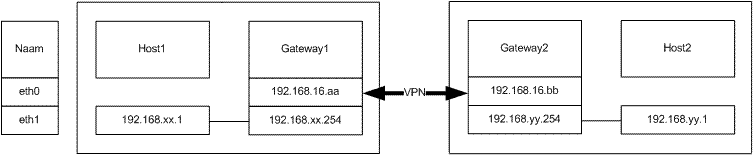
\includegraphics[width=\textwidth]{ipsec}
	\caption{IPSec configuratie.}
	\label{fig:ipsec}
\end{figure}

In deze opstelling blijven enkel de twee gateways verbonden met het bestaande netwerk via de lan0 interface, en zijn de IP-adressen 192.168.16.(aa bb) de originele IP-adressen van je toestel. De VPN-verbinding op de figuur loopt dus over het bestaande 192.168.16/24 netwerk.

Maak op de gateways gebruik van wireshark om alle inkomende en/of uitgaande IP-pakketten te bekijken. Ga steeds na of de IP-pakketten over de juiste headers beschikken (ESP en/of AH) en of de payload al dan niet werd geëncrypteerd. 

\section{Opgave}


\begin{enumerate}
	\textbf {\item Voorzie een veilige IPSec-verbinding tussen de twee clientcomputers. Test eerst uit met ESP zonder AH, daarna met AH zonder ESP.
	Voor deze vraag maak je nog geen gebruik van een combinatie van beide of van tunneling.}

 	\hrulefill
 	
 	Verkorte notatie: x = 192.168.70.1 en y = 192.168.76.1
 	
 	Voer het commando \texttt{setkey -f bestandsnaam} uit, met \textbf{bestandsnaam} de naam van het configuratiebestand waarin volgende instellingen komen.
 	
 	\begin{itemize}
 		\item \textbf{ESP configuratie.}
 		\begin{itemize}
 			\item hilbert
			\begin{lstlisting}
spdflush; -> zit in elk bestand
flush; -> zit in elk bestand
add y x esp 0x01 -m transport -E des-cbc "01234567";
add x y esp 0x02 -m transport -E des-cbc "01234567";
spdadd y x any -P out ipsec esp/transport//require;
spdadd x y any -P in ipsec esp/transport//require;
 			\end{lstlisting}
 			
 			\item fermat
 			
 			\begin{lstlisting}
add y x esp 0x01 -m transport -E des-cbc "01234567";
add x y esp 0x02 -m transport -E des-cbc "01234567";
spdadd x y any -P out ipsec esp/transport//require;
spdadd y x any -P in ipsec esp/transport//require;
 			\end{lstlisting}
 		\end{itemize}
 		
 		
 		
 		\item \textbf{AH configuratie.}
 		 		\begin{itemize}
 			\item hilbert
 			\begin{lstlisting}
add y x esp 0x01 -m transport -A hmac-md5 "0123456789ABCDEF";
add x y esp 0x02 -m transport -A hmac-md5 "0123456789ABCDEF";
spdadd y x any -P out ipsec ah/transport//require;
spdadd x y any -P in ipsec ah/transport//require;
 			\end{lstlisting}
 			
 			\item fermat
 			
 			\begin{lstlisting}
add y x esp 0x01 -m transport -A hmac-md5 "0123456789ABCDEF";
add x y esp 0x02 -m transport -A hmac-md5 "0123456789ABCDEF";
spdadd x y any -P out ipsec ah/transport//require;
spdadd y x any -P in ipsec ah/transport//require;
 			\end{lstlisting}
 		\end{itemize}
 	\end{itemize}
 	

 		
	\textbf {\item  Voortbouwend op de vorige vraag test je nu uit of je het verkeer tussen de clients kan encrypteren en bovendien ook kunt voorzien van de nodige authenticatie. Opnieuw wordt er geen tunneling gebruikt.
	Om dit te realiseren zijn er twee mogelijkheden, eerst encrypteren en dan authenticeren of omgekeerd. Test beide mogelijkheden uit en ga telkens na of er tussen de clients nog communicatie mogelijk is. Wanneer dit niet het geval is, maak je een schets om aan te tonen dat de uitgeteste configuratie niet kan werken.}
	
	\hrulefill
	
	De combinatie waarbij AH eerst gebruikt wordt is onmogelijk. AH zal eerst het bericht authenticeren op basis van de IP header. ESP zal deze IP header overschrijven, waardoor het onmogelijk is om de authenticatie te bevestigen. Eerst ESP, gevolgd door AH zal werken. 
	
	\begin{itemize}
		\item hilbert 
			\begin{lstlisting}
add y x esp 0x01 -m transport -E des-cbc "01234567";
add y x esp 0x02 -m transport -A hmac-md5 "0123456789ABCDEF";.
spdadd y x any -P out ipsec esp/transport//require ah/transport//require;
spdadd x y any -P in ipsec esp/transport//require ah/transport//require;
			\end{lstlisting}
		\item fermat 
			\begin{lstlisting}
add y x esp 0x01 -m transport -E des-cbc "01234567";
add y x esp 0x012 -m transport -A hmac-md5 "0123456789ABCDEF";.
spdadd x y any -P out ipsec esp/transport//require ah/transport//require;
spdadd y x any -P in ipsec esp/transport//require ah/transport//require;
			\end{lstlisting}
	\end{itemize}
	

	
	
	
	
	\textbf {\item  Op de clientcomputers behoud je het authenticatiegedeelte in transportmode. Het is dus niet nodig om het verkeer tussen beide clients te encrypteren.
	Tussen de gateways voorzie je nu bovendien een IPSec-tunnel. Test eerst uit met een AH-tunnel, daarna met een ESP-tunnel. Maak bij iedere opstelling een schets die aantoont of de gevraagde configuratie mogelijk is.}

\hrulefill

Extra notatie: a = 192.168.70.254 en b = 192.168.76.254
	
	\textbf {\item  Net zoals bij de vorige vraag zet je tussen de beide gateways een ESP-tunnel op. Aanvullend zorg je ervoor dat er tussen beide gateways authenticatie gebeurt in transportmode.
	Beide clients maken nog steeds gebruik van AH in transportmode. Test grondig uit en maak opnieuw de nodige schetsen.}
	
	\textbf {\item  Herneem de vorige vraag maar gebruik nu de racoon-daemon voor het aanmaken van de SA's op de clients en op de gateways. Om niet vanaf nul te moeten vertrekken kan je gebruikmaken van dit configuratiebestand. Vergeet niet om het bestand /etc/racoon/psk.txt aan te vullen zodat beide eindpunten over dezelfde sleutel beschikken.
	Ter info: wanneer er geen verkeer optreedt tussen de eindpunten, worden er door racoon geen nieuwe SA's aangemaakt! Je doet er dus goed aan om steeds een console open te houden waar je een ping stuurt naar het andere eindpunt.}
	
	\textbf {\item  Tot slot kan je eens nagaan wat er gebeurt als je tussen de gateways een dubbele tunnel opzet (ESP en AH in tunnelmode). Test uit in welke mate de volgorde een rol speelt en maak opnieuw een schets om na te gaan of het gevraagde enerzijds mogelijk is en anderzijds zinvol is.}
\end{enumerate}


\chapter{PGP}
Dit labo voer je elk afzonderlijk uit op je eigen \textbf{virtuele machine}, dus niet in groep. Maak op je VM drie gewone gebruikers aan: \textit{pgp1, pgp2} en \textit{pgp3}. Alle vollgende opdrachten voer je uit als één van deze gebruikers.
\section{Sleutelbeheer}
	\begin{figure}[h]
	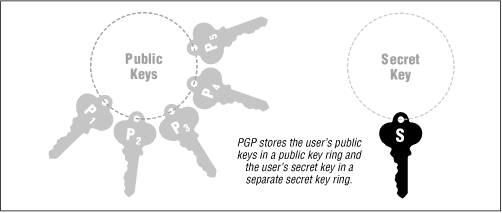
\includegraphics[width=\textwidth]{keyrings}
	\caption{Keyrings}
	\label{fig:keyrings}
\end{figure}
\subsection{Aanmaken sleutels}
\textbf{Maak voor gebruiker \textit{pgp1} drie sleutelparen aan (RSA and RSA, DSA en RSA). Voor gebruikers \textit{pgp2} en \textit{pgp3} maak je telkens twee sleutelparen aan; een RSA and RSA sleutelpaar en een DSA-sleutelpaar. Zorg er voor dat elke sleutel een verschillend ID heeft die de naam van de gebruiker bevat alsook de encryptiemethode. Kies een verschillende geldigheidsperiode voor de sleutels.}


	 Indien gpg nog niet geïnstalleerd is :
	$$\texttt{yum install gpg}$$
	Het kan zijn dat hij de mirrors niet kan resolven, clear de cache dan:
	$$\texttt{yum clean all}$$
	Installeer ook de rng-tools om entropy te genereren:
	$$\texttt{yum install rng-tools}$$
	In de virtual machine kan je nieuwe terminals openen via CTRL + $\vert$ F1 $\vert$ F2 $\vert$ F3 $\vert$ ... $\vert$ F7. Log in op deze verschillende terminals als de drie gebruiker accounts. Behou ook nog een terminal voor de root gebruiker (CTRL + F1 voor root bijvoorbeeld). Run het commando rng-tools in de voorgrond, zodat het random activiteit zal blijven genereren, dit is nodig bij het genereren van sleutels:
	$$\texttt{/usr/sbin/rngd -f -r /dev/urandom}$$
	
	Een sleutel genereren kan met 
	$$\texttt{gpg --gen-key}$$
	Als \textit{pgp1} doe je dit drie keer, telkens met een verschillend algoritme. Als \textit{pgp2} en \textit{pgp3} twee keer: eens met DSA en dan met RSA. 
\begin{itemize}
	\item \textbf{Waarvoor dient de passphrase?} De passphrase dient om de private sleutel te beschermen. Sommige acties op sleutels vereisen ook deze passphrase.
	\item \textbf{Waarom wordt er bij het aanmaken van een sleutel soms naar extra toetsaanslagen gevraagd en soms ook niet?} GPG maakt gebruik van activiteiten zoals toestaanslagen en muisbewegingen (systeemactiviteiten) om entropy te genereren. Gelukkig kan dit vermeden worden door \textit{rngd} te gebruiken.
	\item \textbf{Wat is het verschil tussen "RSA and RSA" en "DSA and Elgamal"?}
\subsection{Exporteren en uitwisselen sleutels}
\textbf{Exporteer al je publieke sleutels naar meerdere bestanden die je aan andere gebruikers kan aanbieden. Exporteer deze in 2 verschillende formaten, waarvan er één geschikt is voor transport via e-mail of publicatie op een webserver.}

Gebruik het volgende commando om één enkele sleutel te exporteren. De variabele \texttt{UNIEKE\_NAAM} bevat een identificatie van de sleutel (bv op basis van Real Name en Comment, of gewoon het ID van de sleutel). 
$$\texttt{gpg --export UNIEKE\_NAAM --output \textasciitilde/outputnaam}$$
Voor leesbare exports gebruik je de \texttt{--armor} optie:
$$\texttt{gpg --armor --export UNIEKE\_NAAM --output \textasciitilde/outputnaam}$$
Het is ook mogelijk om alle sleutels direct te exporten, door geen argument mee te geven aan \texttt{--export}:
$$\texttt{gpg --export --output \textasciitilde/outputnaam}$$
\textbf{Wat is het formaat van deze bestanden?} Zonder de \texttt{--armor} optie hebben de exportbestanden een binair formaat. Deze bestanden uitprinten op een terminal heeft dan ook geen nut. Met de \texttt{--armor} optie ziet het er bijvoorbeeld als volgt uit (ingekort):
\begin{lstlisting}
-----BEGIN PGP PUBLIC KEY BLOCK-----
Version: GnuPG v1.2.1 (GNU/Linux)
Comment: For info see http://www.gnupg.org

mQGiBDkHP3URBACkWGsYh43pkXU9wj/X1G67K8/DSrl85r7dNtHNfLL/ewil10k2
q8saWJn26QZPsDVqdUJMOdHfJ6kQTAt9NzQbgcVrxLYNfgeBsvkHF/POtnYcZRgL
=BMEc
-----END PGP PUBLIC KEY BLOCK-----
\end{lstlisting}

\textbf{Wissel deze bestanden uit met de andere gebruikers (bv. door ze in een gedeelde directory te plaatsen). We gaan er op dit ogenblik van uit dat sleutels die op deze manier zijn verkregen, volledig te vertrouwen zijn.} 

De eenvoudigste manier is om als root gebruiker de bestanden te kopieëren naar de root folder van elke gebruiker (gebruik hiervoor de terminal die voor de root gebruiker beschikbaar is).
$$\texttt{cp /home/pgp1/exportbestand /home/pgp2/exportbestand\_pgp1}$$
\end{itemize}

\subsection{Toevoegen sleutels}
\textbf{Voeg voor elke gebruiker de verkregen publieke sleutels toe aan zijn publieke sleutelhanger. Verifieer of ze wel zijn opgenomen.}

Een sleutel importeren kan met 
$$\texttt{gpg --import bestandsnaam}$$
Dit commando zal ook specificeren hoeveel publieke sleutels er zijn toegevoegd. Om een lijst van alle sleutels op te vragen gebruik je
$$\texttt{gpg --list-key}$$

\textbf{Verwijder één van de sleutels uit de sleutelhanger. Controleer en voeg de sleutel nadien weer toe.}

Een sleutel verwijderen kan met 
$$\texttt{gpg --delete-key sleutelID}$$

\subsection{Wijzigen sleutels}
\textbf{Wijzig één van de sleutels: verander de passeerzin.}
Een sleutel wijzigen kan met
$$\texttt{gpg --edit-key sleutelID}$$
Na het uitvoeren van dit commando zit je in een menu. Met \textit{help} kan je alle mogelijke opties ophalen. Een passphrase veranderen kan met \textit{passwd}.

\subsection{Vertrouwen sleutels}
\begin{itemize}
	\item \textbf{Controleer de sleutels en de handtekeningen die er bij horen.}
	\item \textbf{Verifieer de fingerprint van de sleutels bij de verschillende gebruikers.}
	
	Gebruik \texttt{gpg --verify sleutelID}
	\item \textbf{Zorg er voor dat al de sleutels in de sleutelhangers volledig vertrouwd worden, indien dit nog niet het geval zou zijn.}
	
	Een sleutel vertrouwen kan terug met \texttt{gpg --edit-key sleutelID}.
	In het menu gebruik je nu \texttt{trust}, en geef je ultimate trust aan elke sleutel. Hiervoor moet dus elke keer het gpg commando met de \texttt{--edit-key} optie uitgevoerd worden voor elke sleutel.
	\item \textbf{Teken voor elke gebruiker de eigen sleutels en die van de andere gebruikers van wie de sleutel vertrouwd wordt.}
	
	Gebruik hiervoor de \texttt{sign} optie in de \texttt{--edit-key} menu.
\end{itemize}

\section{Encrypteren en decrypteren van bestanden}
\begin{figure}[h]
	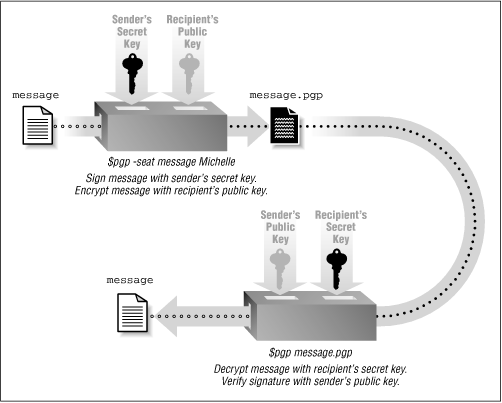
\includegraphics[width=\textwidth]{encrypting}
	\caption{Encryptie.}
	\label{fig:encrypting}
\end{figure}
\subsection{Lokaal encrypteren en decrypteren}
\textbf{Maak als gebruiker \textit{pgp1} vijf korte tekstbestanden aan om ze nadien aan de andere gebruikers over te maken. Encrypteer deze bestanden als volgt: }
\begin{enumerate}
	\item \textbf{het eerste bestand encrypteer je door middel van conventionele encryptie op twee manieren:
		de eerste keer met het default algoritme,
		de tweede keer geef je zelf het algoritme op (bv. AES256). }
	Het default algoritme is CAST5. Het volgende commando zal een bestand encrypteren met dit algoritme:
	$$\texttt{gpg --encrypt bestand1}$$
	Er zal een prompt komen voor User IDs, laat dit voorlopig leeg. Het uitvoerbestand zal \texttt{bestand1.gpg} zijn. Dit zullen ook de bestanden zijn die moeten verzonden worden over een netwerk naar de begunstigde.
	
	
	Zelf aan algoritme meegeven kan met de \texttt{--cipher-algo} optie:
	$$\texttt{gpg --encrypt --cipher-algo AES256 bestand1}$$
	
	\item \textbf{het tweede bestand encrypteer je zodat alleen gebruiker pgp2 het bestand kan decrypteren.}
	
	Hier wordt ervan uitgegaan dat de naam van de sleutels van de gebruiker pgp2, zelf ook de string "pgp2" bevatten.
	$$\texttt{gpg --encrypt --recipient pgp2 bestand2}$$
	
	\item \textbf{het derde bestand encrypteer je zodat dit door gebruikers pgp2 en pgp3 kan ontcijferd en gelezen worden. Zorg dat de encryptie met een ander dan het default algoritme gebeurt.}
	$$\texttt{gpg --encrypt --cipher-algo AES256 bestand3}$$
	Vul nu in de prompt twee User IDs in, namelijk die van pgpp2 en pgp3 (op aparte lijnen).
	
	\item \textbf{het vierde bestand encrypteer je zodat gebruiker pgp2 hem niet zonder meer kan opslaan op zijn vaste schijf.}
	
	???
	
	\item \textbf{het vijfde bestand encrypteer je conventioneel maar het resultaat is in radix64.}
\end{enumerate}

\textbf{Veeg de originele plaintextbestanden uit. Probeer nu de plaintext te herstellen uitgaande van de ciphertext van elk bestand. Controleer wat er al dan niet nog kan gebeuren}

\subsection{Remote decrypteren}
\textbf{Wissel al de geëncrypteerde bestanden uit met de gebruikers pgp2 en pgp3. Decrypteer alle ontvangen bestanden. Beschrijf in elk van de gevallen wat er gebeurt.}
Een bestand decrypteren kan met:
$$\texttt{gpg --decrypt bestandsnaam}$$
Indien dit bestand bedoeld was voor de huidige gebruiker, dan zal hij deze kunnen decrypteren, en zal de inhoud van het bestand naar de console geschreven worden. Is dit niet zo zal er een foutmelding komen dat de juiste sleutel niet beschikbaar is.

\section{Sleutelbeheer}

\chapter{Sendmail}
Dit labo bestaat uit 2 delen: in het eerste deel maken we een basisconfiguratie aan voor sendmail, die we in het tweede deel gebruiken om de mogelijkheden van S/MIME even uit te testen. Binnen elke groep zal één virtuele machine dienst doen als sendmail-server. Deze server zal verantwoordelijk zijn voor jouw domein. Vooraleer echt aan de slag te gaan, doe je best het volgende: 
\begin{itemize}
	\item Voor dit labo start je best met een 'cleane' VM. Zet indien nodig de backup van je virtuele machine terug. Controleer zeker volgende instellingen: 
	\begin{itemize}
		\item De virtuele netwerkinterface is in bridge modus verbonden met de fysieke netwerkadapter en heeft een IP-adres binnen jouw netwerkrange (192.168.x.2 of 192.168.x.3).
		\item De default gateway is ingesteld naar jouw gateway (192.168.x.254).
		\item Je eigen DNS-servers staan ingesteld in /etc/resolv.conf.
		\item \texttt{firewalld} is \textbf{niet} geïnstalleerd (yum remove firewalld + reboot).
		\item Om problemen te voorkomen schakel je ook best SELinux uit.
	\end{itemize}
	\item Maak eventueel een extra backup van je VM die je indien nog snel kan terugplaatsen.
	\item Maak een kopie van het configuratiebestand sendmail en plaats dit in de homedirectory van de root-gebruiker (\texttt{cp /etc/mail/sendmail.mc ~/sendmail.mc.bak}).
	\item Zorg dat je over twee gebruikers beschikt: \textit{tiwi1} en \textit{tiwi2} met hetzelfde wachtwoord als \textit{root}
\end{itemize}
Aangezien er twee DNS-domeinen per tafel zijn voorzien, kan je voor het uittesten van sendmail gebruikmaken van het naburige domein. E-mailverkeer treedt dan ook voornamelijk op tussen deze twee domeinen, maar is ook mogelijk met andere domeinen.
\section{Configuratie sendmail}
\subsection{Basisconfiguratie}
\textbf{Voor de basisconfiguratie van sendmail kan je starten van dit} (wordt gegeven) \textbf{ configuratiebestand.
Let op: hier en daar moet je nog iets aanpassen! Ga na of je nu met deze basisconfiguratie via jouw mailserver een mail kan versturen naar een lokale gebruiker.
Controleer ook of je een mail kan versturen naar een lokale gebruiker van het andere domein.
Een e-mail versturen kan je m.b.v. het commando mail -v (of -vv om nog meer informatie te verkrijgen). Zorg er tenslotte voor dat post die bestemd is voor lokale gebruikers niet meer wordt rondgestuurd naar eventuele andere mailservers.}

Wij gebruiken de gateway als mailserver. Dus alle configuratie gebeurd dan ook op dat toestel. Installeer eerst de software:
$$\texttt{yum install sendmail sendmail-cf mailx m4}$$
Het sendmail.mc bestand dat we gekregen hebben is grotendeels goed, enkel twee lijnen moeten aangepast worden:
\begin{lstlisting}
MASQUERADE_AS(groep20.iii.hogent.be)dnl
GENERICS_DOMAIN('groep20.iii.hogent.be')dnl
\end{lstlisting}


Voeg bij de primaire DNS (NIET de gateway) het volgende \textbf{MX} (mail exchange) record toe in het zonebestand (\texttt{/var/named/groep20.iii.hogent.be}) en herstart hierna de \textbf{named} service:
$$\texttt{ivoryVM IN MX 10 192.168.70.2}$$
$$\texttt{service named restart}$$
Terug op de gateway in het bestand \texttt{/etc/mail/local-host-names}:
\begin{lstlisting}
ivoryVM.groep20.iii.hogent.be
groep20.iii.hogent.be
FEATURE('use_cw_file')
\end{lstlisting}
Verstuur een email met:
$$\texttt{[root@ivoryVM]: mail -s "Onderwerp"\space tiwi1@hilbertVM < /dev/null}$$
en bekijk deze met:
$$\texttt{root@hilbertVM}: cat /var/mail/tiwi1$$

\subsection{Aliases}
\textbf{Zorg er voor dat tiwi1 een alias is voor jouwvoornaam.jouwnaam@jouwdomein.iii.hogent.be.
 Doe hetzelfde voor jouw collega, maar dan met gebruiker tiwi2. Welke bestanden heb je aangepast en welke informatie heb je aan die bestanden toegevoegd? 
 Test deze instellingen eerst uit vanuit je lokale domein, en nadien vanuit een ander domein.}

In het bestand \texttt{/etc/aliases}:
\begin{lstlisting}
xandro.vermeulen@groep20.iii.hogent.be: tiwi1@ivoryVM
bert.desaffel@groep20.iii.hogent.be: tiwi2@hilbertVM
\end{lstlisting}
Hierna moet het commando \texttt{newaliases} uitgevoerd worden, zodat sendmail op de hoogte is van deze aliases. Vanaf dan kunnen de aliases gebruikt worden.

\textbf{Wat moet je aanpassen als je ook mails wenst te versturen vanaf \\
jouwvoornaam.jouwnaam@jouwdomein.iii.hogent.be?}
\subsection{IMAP en/of POP3}
\textbf{ Om via IMAP en/of POP3 je mails te kunnen ophalen kan je gebruikmaken van dovecot.
Installeer indien nodig dovecot op je VM (via yum).
	
Voor een correcte werking van dovecot overschrijf je het configuratiebestand (/etc/dovecot/dovecot.conf) door dit bestand.
De bestanden /etc/dovecot/conf.d/10-auth.conf en /etc/dovecot/conf.d/10-ssl.conf vervang je respectievelijk door dit en dit bestand.
	
Lees de man-pagina van het commando mail en gebruik dit commando met bijhorende opties om op een ander toestel jouw persoonlijke berichten via POP3 van de mailserver af te halen. Beantwoord een ontvangen bericht en ga na of alles correct werkt. }

Gewoon de bestanden kopieren, daarna:
\begin{lstlisting}
yum install dovecot
service dovecot start 
\end{lstlisting}

\section{S/MIME}
\subsection{Configuratie e-mail client}
\textbf{ Om S/MIME te kunnen gebruiken en uittesten is het noodzakelijk een e-mail-client te gebruiken die dit aankan. In dit labo maken we hiervoor gebruik van Mozilla Thunderbird.
	
	Configureer op beide fysieke toestellen (gateway en client1) Thunderbird voor de gebruikers tiwi1 en tiwi2.
	Kies bijvoorbeeld tiwi1 op de gateway en tiwi2 op de primaire DNS-server.
	
	Probeer je berichten op te halen via IMAP of POP3.
	Merk op dat dovecot hiervoor correct geconfigureerd moet zijn!
	Stuur een mail naar de andere gebruiker en controleer of alles werkt. }
\subsection{Certificaat}
\textbf{ Om een digitale handtekening toe te voegen aan e-mails, of e-mails te kunnen encrypteren hebben we opnieuw een certificaat nodig.
	Vraag via onze CA (link) een certificaat aan en voeg dit certificaat toe in Thunderbird.
	Voor deze vraag moet je geen CSR genereren, maar mag je het online formulier gebruiken.}
\subsection{Authenticatie en/of encryptie}
\textbf{Verzend naar je collega een bericht dat je probeert te encrypteren.
	Waarom lukt dat niet? Waarom lukt dit wel als je naar jezelf een e-mail stuurt?
	
	Verzend nu naar elkaar een ondertekend bericht. Bij ontvangst wordt het gebruikte certificaat automatisch geïnstalleerd. Controleer dit en verifieer ook de vingerafdruk.
	
	Probeer nu opnieuw een bericht te encrypteren en naar je collega te versturen. Voeg eventueel ook een handtekening toe aan je bericht.}
\subsection{Opslag mails op server}
\textbf{ Alle mails worden op de sendmail-server opgeslagen in de directory /var/spool/mail/.
	Bekijk de inhoud van deze bestanden.
	Wat is het formaat van een mail met authenticatie en/of encryptie?}

\chapter{PAM}
Dit labo voer je elk afzonderlijk uit op je eigen \textbf{virtuele machine}, dus niet in groep. Om dit labo te kunnen uitvoeren moeten de globale configuratieinstellingen in \texttt{/etc/pam.d} worden aangepast. Neem daarom bij het begin van het labo een backup van je virtuele harde schijf. Aan het einde van dit labo plaats je deze kopie terug! 

\accentuate{Opgelet: het aanpassen van de configuratie doe je als root-gebruiker en \textbf{TREEDT ONMIDDELLIJK IN WERKING}. \textbf{Blijf dus op elk moment op minstens 1 console als root-gebruiker ingelogd} voor het geval er iets verkeerd zou gaan!}

Maake 2 extra lokale gebruikers aan met volgende eigenschappen:
\begin{itemize}
	\item pam1: UID $>$ 1000 en GID $>$ 1000
	\item pam2: UID $<$ 1000 en GID $<$ 1000
	\item beide gebruikers hebben een wachtwoord.
\end{itemize}
Voordat je een gebruiker aanmaakt, controleer je best of het UID dat je wil instellen nog niet door een andere gebruiker ingenomen is. 
\begin{lstlisting}
cat /etc/passwd | cut -d ':' -f3 // om reeds gebruikte UIDs te zien
cat /etc/groups | cut -d ':' -f3 // om reeds gebruikte GIDs te zien

adduser pam1 -u 1500
groupmod -g 1600 pam1 
passwd pam1

adduser pam2 -u 500
groupmod -g 600 pam2 
passwd pam2
\end{lstlisting}

\section{Pamtester}
Pamtester is een tool die werd ontwikkeld voor het testen van de PAM-configuratie. Meer informatie over Pamtester en over het gebruik ervan kun je vinden in de bijgevoegde man-pages. De installatie gebeurt als volgt:
$$\texttt{yum install pamtester}$$
Na deze stappen kun je de tester gewoon gebruiken. Probeer hem ook eens uit, zodat je weet hoe hij werkt. 

\section{Opdrachten}
\begin{enumerate}
	\item \textbf{Configureer PAM zodat de meeste modules debug-informatie wegschrijven.}
	
	Het bestand \texttt{/etc/pam.d/system-auth} aanpassen, zodat elke lijn eindigt met 'debug'.
	\begin{lstlisting}

auth     required   pam_env.so debug
auth     sufficient pam_unix.so nullok try_first_pass debug
auth     requisite  pam_succeed_if.so uid >= 500 debug
auth     required   pam_deny.so debug
		
account  required   pam_unix.so debug
account  sufficient pam_succeed_if.so uid < 500 debug
account  required   pam_permit.so debug
		
password requisite  pam_pwquality.so try_first_pass retry=3 debug
password sufficient pam_unix.so md5 ... use_authtok debug
password required   pam_deny.so debug
		
session  required   pam_limits.so debug
session  required   pam_unix.so debug
	\end{lstlisting}
	\textbf{In welk(e) bestand(en) komt deze informatie terecht?}
	Je kan logbestanden opvragen met 
	$$\texttt{journalctl -f -l SYSTEM\_FACILITY=10}$$
	\item \textbf{Pas de configuratie aan zodat een gebruiker 5 kansen krijgt om een aanvaardbaar nieuw wachtwoord in te geven bij het wijzigen van zijn wachtwoord.}
	
	Verander lijn 8 van het bestand \texttt{/etc/pam.d/system-auth} zodat retry op 5 staat i.p.v. 3.
	\begin{lstlisting}
password requisite  pam_pwquality.so try_first_pass retry=5 debug
	\end{lstlisting}
	\item \textbf{Pas het systeem aan zodat gebruikers met UID $>$ 1000 (bv. pam1) niet kunnen inloggen en die met een UID $<$ 1000 (bv. pam2) wel. Test uit met de nieuw aangemaakte gebruikers.}

	Voeg deze twee lijnen toe in de bestanden \texttt{/etc/pam.d/su} en \texttt{/etc/pam.d/login} in hun respectievelijke stack. Waar dat deze lijnen komen maakt niet zoveel uit, als het maar zeker niet onder de pam module \texttt{pam\_deny.so} staat:
	\begin{lstlisting}
auth    requisite pam_succeed_if.so uid < 1000
account requisite pam_succeed_if.so uid < 1000
	\end{lstlisting}

	\item \textbf{Bij systeemonderhoud is het wenselijk dat niet-root-gebruikers zich voor een bepaalde tijd niet kunnen aanmelden; pas dit toe voor ssh en voor login. Zorg er bovendien voor dat gebruikers die toch proberen in te loggen een passende boodschap te zien krijgen.}
	
	In de bestanden \texttt{/etc/pam.d/sshd} en \texttt{/etc/pam.d/login} staat al de nodige lijn om deze module in te schakelen, namelijk:
	\begin{lstlisting}
auth required pam_nologin.so
	\end{lstlisting}
	Deze module wordt echter pas uitgevoerd indien er een bestand \texttt{/etc/nologin} bestaat. In dit bestand staat ook de boodschap die getoond zal worden indien een niet-root gebruiker zal proberen inloggen.

	\item \textbf{Configureer PAM zodat gebruiker pam1 enkel kan inloggen vanop de computer van je collega.}
	
	Voeg de volgende lijn toe in het bestand \texttt{/etc/pam.d/system-auth}:
	\begin{lstlisting}
auth requisite pam_access.so debug
	\end{lstlisting}
	Deze module kijkt in het bestand \texttt{/etc/security/access.conf}. Vul de inhoud aan met (vanuit perspectief van hilbertVM):
	\begin{lstlisting}
+ : pam1 : 192.168.70.2
- : pam1 : 192.168.70.3
	\end{lstlisting}
	\item \textbf{Configureer PAM zodanig dat root uitsluitend nog kan inloggen vanop tty4. Vergeet niet om root nog steeds ingelogd te houden op 1 andere console!}
	
	Ook hier staat de nodige pam module (\texttt{pam\_securetty}) al ingesteld in de nodige bestanden. Enkel het bestand \texttt{/etc/securetty} moet aangepast worden zodat deze enkel tty4 bevat. Maak eerst een backup met 
	$$\texttt{cp /etc/securetty /etc/securetty.bak}$$
	en verwijder daarna alles behalve tty4 uit \texttt{/etc/securetty}.

	\item \textbf{Zorg ervoor dat lokaal inloggen en inloggen via ssh enkel mogelijk is op maandagen van 10 tot 12. Uiteraard pas je deze tijden aan om te kunnen testen.}
	
	Voeg volgende lijn toe in \texttt{/etc/pam.d/sshd} en \texttt{/etc/pam.d/login}:
	\begin{lstlisting}
auth required pam_time.so
	\end{lstlisting}

	Pas dan volgende instelling toe in het bestand \texttt{/etc/security/time.conf}:
	\begin{lstlisting}
login;*;*;Th1000-1200
sshd;*;*;Th1000-1200
	\end{lstlisting}
	
	\item \textbf{Zorg ervoor dat lokaal inloggen en inloggen via ssh enkel mogelijk is op maandagen en vrijdagen voor pam1 en pam2. Uiteraard pas je deze dagen aan om te kunnen testen.}
	
	Terug het bestand \texttt{/etc/security/time.conf} aanpassen:
	\begin{lstlisting}
login; * ; pam1 | pam2 ; MoFr0000-2400
sshd ; * ; pam1 | pam2 ; MoFr0000-2400
	\end{lstlisting}
	\item \textbf{Wat gebeurt er indien iemand zich aanmeldt via een service die niet voorkomt in de directory \texttt{/etc/pam.d}?}
\end{enumerate}

\chapter{iptables}
Tijdens dit labo werk je alleen aan een toestel. Dit labo voer je volledig uit op je \textbf{virtuele machine}, voer dus geen commando's uit op de gateway of op client1. Plaats eventueel bij het begin van dit labo een backup van je virtuele disk terug. Vergeet niet om firewalld te verwijderen mocht dit nog geïnstalleerd zijn (\texttt{yum remove firewalld}).

Zorg er voor dat je \textbf{NIET} bent ingelogd als gewone gebruiker maar als \emph{root} (dus ook geen \texttt{su - }!!).
\section{Vooraf} 
Implementeer volgende firewallregels met behulp van het \texttt{iptables}-commando. Informatie over de poorten kan je vinden in \texttt{/etc/services}.
Test uit op je eigen machine en ook via je buren. Vergeet niet dat je telkens de instellingen kan nakijken met de list-vlag van het \texttt{iptables}-commando.

Hou ook rekening met volgende opmerkingen:
\begin{itemize}
	\item Het is zeer handig en \textbf{tijdbesparend} als je alle regels opslaat in een script!! Dit laat ook toe om voor bepaalde dns-namen of ip-adressen een variabele (inderdaad: een shell-variabele!) te gebruiken die je in het begin van het script initialiseert.
    \item Je kan in de opgestelde regels zowel ip-adressen als dns-namen gebruiken. Het gebruik van ip-adressen geniet de voorkeur, omdat op die manier je firewall blijft functioneren los van het feit of de nameserver werkt/bereikbaar is of niet.
\end{itemize}
    

Om na te gaan welke poorten er op een toestel open staan, kan je gebruikmaken van de nmap-tool. Meer informatie over het gebruik van het commando \texttt{nmap} kan je vinden in de man-pages.

Via iptables kan je zowel stateless als stateful regels toevoegen. Voor dit labo mag je \textbf{alle regels stateless} toevoegen, tijdens het labo firewalls (inhaalweek) zullen we ook met stateful regels werken. 

Belangrijk: Indien je om \textbf{10u45} nog niet aan vraag 8 bent gekomen, begin je op dat moment zeker bij 8 (Opgave deel 2). Ben je klaar met de tweede reeks voor het einde van het labo, dan werk je de eerste reeks opgaven verder af. 

\section{DEEL1 - Default policy ACCEPT}
Bij de volgende 9 opgaven is het de bedoeling dat je de standaard ingestelde \textbf{policy (ACCEPT)} niet verandert.

Zorg er ook voor dat bij het toevoegen van een nieuwe regel alle tevoren ingestelde regels blijven gelden !!
\begin{enumerate}
	\item     Zorg er voor dat je een ftp-connectie kan leggen met je machine. Installeer indien nodig een ftp server op je virtuele machine (\texttt{yum install pure-ftpd}).
    De service starten kan via \texttt{systemctl start pure-ftpd}. Merk op dat je op de ftp-server enkel kan inloggen als niet-root gebruiker.
	Stel regels op die er voor zorgen dat geen enkele computer een ftp-verbinding kan maken met jouw virtuele machine.
	\begin{lstlisting}[escapeinside={(*}{*)}]
iptables -A INPUT -p tcp (*$--$*)dport 20 -j DROP
iptables -A INPUT -p udp (*$--$*)dport 20 -j DROP
iptables -A INPUT -p tcp (*$--$*)dport 21 -j DROP
iptables -A INPUT -p udp (*$--$*)dport 21 -j DROP
	\end{lstlisting}
	\item     Laat nadien selectief alleen ftp vanaf je eigen vm naar jezelf toe. Test zeer kritisch: gebruik zowel localhost, de naam, het ip-adres als de loopback van je machine.
	\begin{lstlisting}[escapeinside={(*}{*)}]
iptables -I INPUT -p tcp -s 127.0.0.1 (*$--$*)dport 20 -j ACCEPT
iptables -I INPUT -p udp -s 127.0.0.1 (*$--$*)dport 20 -j ACCEPT
iptables -I INPUT -p tcp -s 127.0.0.1 (*$--$*)dport 21 -j ACCEPT
iptables -I INPUT -p udp -s 127.0.0.1 (*$--$*)dport 21 -j ACCEPT
	\end{lstlisting}
	\item     Zorg er nu voor dat je een telnet-connectie kan leggen met je virtuele machine. Installeer hiervoor xinetd (\texttt{yum install xinetd}) en telnet-server (\texttt{yum install telnet-server}). Maak bovendien een configuratiefile \texttt{telnet} aan in \texttt{/etc/xinetd.d}. De inhoud van dit bestand vind je hier.
   
	Zorg ook dat er op jouw virtuele machine een webserver draait.

	Stel nadien dezelfde twee regels in (cfr. 1 en 2) voor de protocols www en telnet.
	\begin{lstlisting}[escapeinside={(*}{*)}]
iptables -A INPUT -p tcp (*$--$*)dport 80 -j DROP
iptables -A INPUT -p udp (*$--$*)dport 80 -j DROP
iptables -A INPUT -p tcp (*$--$*)dport 23 -j DROP
iptables -A INPUT -p udp (*$--$*)dport 23 -j DROP
iptables -I INPUT -p tcp -s 127.0.0.1 (*$--$*)dport 80 -j ACCEPT
iptables -I INPUT -p udp -s 127.0.0.1 (*$--$*)dport 80 -j ACCEPT
iptables -I INPUT -p tcp -s 127.0.0.1 (*$--$*)dport 23 -j ACCEPT
iptables -I INPUT -p udp -s 127.0.0.1 (*$--$*)dport 23 -j ACCEPT
	\end{lstlisting}

	\item     Maak nu gebruik van de optie \texttt{multiport} om al de vorige regels te groeperen. Meer informatie over deze optie vind je in de man-pages van \texttt{iptables-extensions}.
	\begin{lstlisting}[escapeinside={(*}{*)}]
iptables -I INPUT -p tcp -s 127.0.0.1 
	 -m multiport (*$--$*)dports 20, 21, 23, 80 -j ACCEPT
iptables -I INPUT -p udp -s 127.0.0.1 
	 -m multiport (*$--$*)dports 20, 21, 23, 80 -j ACCEPT
iptables -I INPUT -p tcp 
	 -m multiport (*$--$*)dports 20, 21, 23, 80 -j DROP
iptables -I INPUT -p udp 
	 -m multiport (*$--$*)dports 20, 21, 23, 80 -j DROP
		\end{lstlisting}
		
	\item     Ga voor het telnet-protocol na wat de effectverschillen zijn tussen de opties \texttt{DROP} en \texttt{REJECT} bij het instellen van de regels.
	Bij REJECT kan je ook zelf kiezen uit een aantal \texttt{icmp-type 3} foutboodschappen. Test uit.
\begin{lstlisting}[escapeinside={(*}{*)}]
iptables -I INPUT -p tcp (*$--$*)dport 23 -j REJECT 
	 (*$--$*)reject-with icmp-port-unreachable
\end{lstlisting}

	\item     Zorg ervoor dat er op geen enkele poort boven 1024 informatie kan verstuurd worden naar moore.iii.hogent.be.
    Test bijvoorbeeld dat http wel werkt, maar dat de tomcat-server op poort 8080 niet te bereiken is.
\begin{lstlisting}[escapeinside={(*}{*)}]
iptables -I OUTPUT -d 192.168.134.8 -p tcp 
	 -m multiport (*$--$*)dports 1025:65535 -j REJECT
iptables -I OUTPUT -d 192.168.134.8 -p udp 
	 -m multiport (*$--$*)dports 1025:65535 -j REJECT
\end{lstlisting}
	\item     Maak dat je eigen machine niet kan ge\emph{ping}d worden. Dit kan je verwezenlijken op verschillende manieren: langs ingangszijde geen aanvragen toelaten, langs uitgangszijde geen antwoord sturen. Probeer beide mogelijkheden uit.
\begin{lstlisting}[escapeinside={(*}{*)}]
# Geen aanvragen toelaten
iptables -I INPUT -p icmp --icmp-type echo-request -j REJECT
# Geen antwoorden sturen
iptables -I OUTPUT -p icmp  --icmp-type echo-reply -j REJECT
\end{lstlisting}
\end{enumerate}


\section{DEEL2 - Default policy DROP}

Aan dit gedeelte start je ten laatste om 10u45. Het oplossen van deze reeks opgaven is belangrijk als voorbereiding voor de volgende sessies van het labo firewalls.

Bij de volgende opgaven is het de bedoeling dat je de standaard ingestelde policy verandert in DROP.
\begin{lstlisting}
iptables -p INPUT DROP
iptables -p FORWARD DROP
iptables -p OUTPUT DROP
\end{lstlisting}
Controleer op meerdere manieren of dit het gewenste effect heeft !!
\begin{enumerate}
	\item[8.]    Zorg er in eerste instantie voor dat je eigen machine in staat is om DNS-namen op te vragen. Controleer met dig (vb. dig a www.google.be).
	\begin{lstlisting}[escapeinside={(*}{*)}]
iptables -I OUTPUT -p udp (*$--$*)dport 53 -j ACCEPT
iptables -I INPUT  -p udp (*$--$*)dport 53 -j ACCEPT
iptables -I OUTPUT -p udp (*$--$*)sport 53 -j ACCEPT
iptables -I INPUT  -p udp (*$--$*)sport 53 -j ACCEPT
	\end{lstlisting}
	\item[9.]  Natuurlijk moet je van op je eigen machine ook nog de webpagina's van http(s)://www.ugent.be kunnen opvragen. Pas je firewall aan en test eventueel uit met behulp van het commando curl of wget.
	\begin{lstlisting}[escapeinside={(*}{*)}]
iptables -I OUTPUT -p tcp -d 157.193.43.50 (*$--$*)dport 80 -j ACCEPT
iptables -I INPUT  -p tcp -d 157.193.43.50 (*$--$*)dport 80 -j ACCEPT
iptables -I OUTPUT -p tcp -d 157.193.43.50 (*$--$*)dport 80 -j ACCEPT
iptables -I INPUT  -p tcp -d 157.193.43.50 (*$--$*)dport 80 -j ACCEPT
	\end{lstlisting}
	\item[10.]    Stel nu een regel op die het mogelijk maakt om je eigen machine als webserver te gebruiken. Laat dit controleren door een van je buren.
	\begin{lstlisting}[escapeinside={(*}{*)}]
iptables -I INPUT  -p tcp -d 192.168.70.3 (*$--$*)dport 80 -j ACCEPT
iptables -I OUTPUT -p tcp -s 192.168.70.3 (*$--$*)dport 80 -j ACCEPT

	\end{lstlisting}
	\item[11.]    Stel nu regels op die het mogelijk maken om je eigen machine als FTP-server te kunnen laten gebruiken: je machine moet door een ftp-client bij je buur kunnen gebruikt worden om er bestanden van op te halen en er op te plaatsen; gebruik hiervoor een van de gewone tiwi-gebruikers.
    In welke mode moet het ftp-commando een connectie leggen opdat de firewallinstellingen effect zouden hebben? Waarom?

    Opmerking: Om FTP in active mode te gebruiken geef je de optie -A mee: ftp -A hostname.

    Ga na of je effectief ook bestanden kan uitwisselen.
	\item[12.]     Tracht alle (normaal 6) regels die je hebt ingesteld in de twee vorige punten 10 en 11 te combineren tot twee regels.

	\item[13.]    Vanuit je machine moet je in staat zijn om naar andere toestellen te pingen. Zorg er bovendien voor dat je eigen machine niet reageert op ping-aanvragen van andere machines.
\end{enumerate}




\chapter{Firewall}
De bedoeling van dit labo is een firewall op te zetten met een gedemilitariseerde zone (DMZ) en een intern netwerk.
Deze opdracht wordt uitgevoerd in groepen van 4, de indeling van de groepen vind je hier.

Elke groep maakt een opstelling met 4 PC's: een externe router (RE), een interne router (RI), een bastion host (BH) en een client in het interne netwerk (CL).
Figuur \ref{fig:9_opstelling} toont de volledige opstelling voor één groep.
\begin{figure}[ht]
	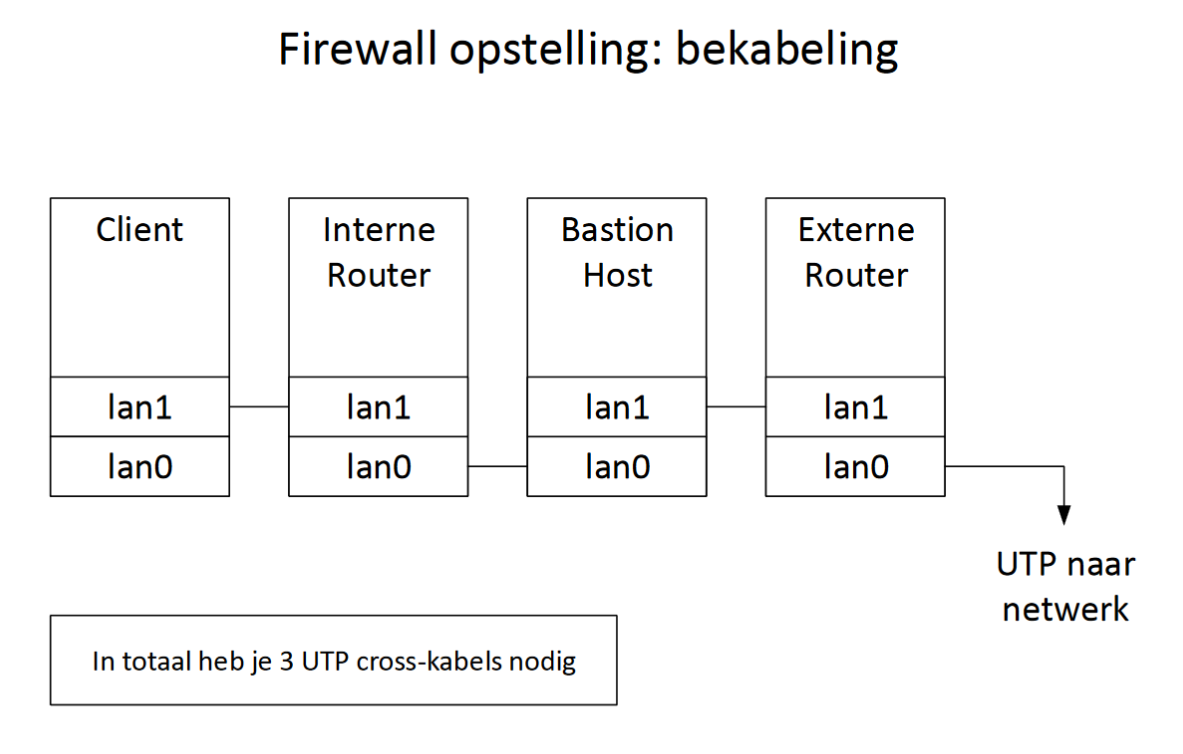
\includegraphics[width=\textwidth]{9_opstelling}
	\caption{Opstelling voor één groep.}
	\label{fig:9_opstelling}
\end{figure}
Let in elk geval ook op de manier waarop de toestellen met elkaar zijn verbonden.

Welk toestel binnen jouw groep zal fungeren als RE, BH, RI en CL kan je hier vinden per lokaal: 2.031 en 2.035.
Een overzicht van alle IP-adressen voor jouw groep vind je op figuur \ref{fig:9_ipaddr}.
\begin{figure}[ht]
	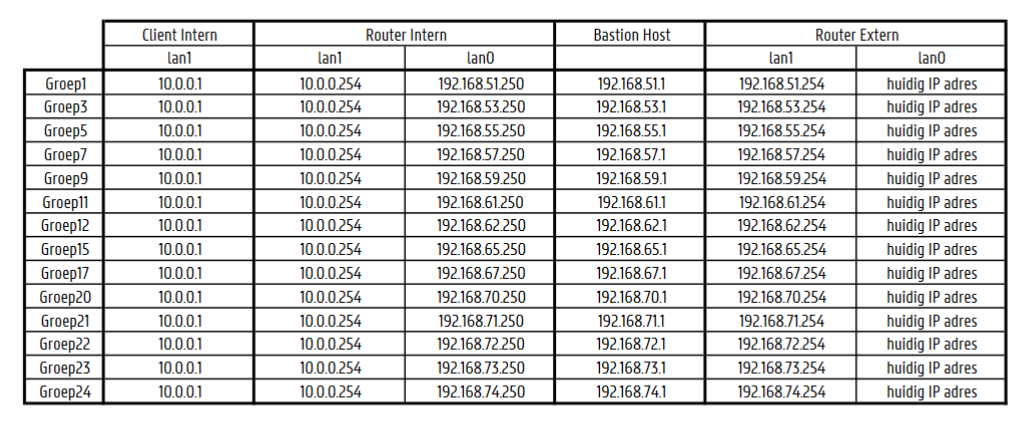
\includegraphics[width=\textwidth]{9_ipaddr}
	\caption{IP-adressen voor elke opstelling.}
	\label{fig:9_ipaddr}
\end{figure}
\section{Routing}

Zorg er in eerste instantie voor dat de routing correct werkt:
\begin{itemize}
    \item Sluit de nodige netwerkkabels aan, en maak overal gebruik van statische IP-adressen, bij voorkeur via ifcfg-bestanden.
    \item Om de route naar de DMZ te verspreiden, zal de externe \textbf{router (RE)} gebruikmaken van een RIPv2-router (via Quagga).
    \item De \textbf{bastion host (BH)} fungeert als bridge, zodat hij in de DMZ verbonden is met zowel de interne als externe router.
    \item De \textbf{interne router (RI)} maakt gebruik van NAT om het interne netwerk te maskeren.
\end{itemize}


De \textbf{externe router} is verbonden met een extern netwerk dat zal fungeren als het \emph{internet}.
Dit is het netwerk waar alle computers zijn op aangesloten die niet in de testopstelling zijn betrokken, zo ook intranet.iii.hogent.be en moore.iii.hogent.be (192.168.16.8).
Het internet op de externe router moet je aansluiten op \textbf{lan0}, dus op de interface waarmee de machine in de normale toestand met het net is verbonden.
Om de route naar de DMZ te verspreiden naar alle andere externe routers, alsook naar moore.iii.hogent.be, zal de externe router gebruikmaken van een \textbf{RIPv2}-router (via Quagga).

De \textbf{bastion host} bevindt zich in de DMZ.
De bastion host fungeert als bridge, zodat hij in de DMZ ook verbonden is met zowel de interne als met de externe router.
Hij zal ook dienst doen als nameserver, als webserver, en als proxyserver voor HTTP en HTTPS (zie verder).

De \textbf{interne router} verbindt het interne netwerk met de DMZ. Op het interne netwerk is één pc aangesloten die dienst doet als testclient (CL).

De DMZ is rechtstreeks bereikbaar van overal op het ''internet'' maar maskeert het interne netwerk.
Dat betekent dat geen enkele computer op het interne netwerk (o.a. de testclient CL) bereikbaar is van buiten, ook niet vanaf de DMZ.
Het private netwerk 10.0.0.0/8 moet dus gemaskeerd worden met behulp van NAT.
Voor de configuratie van NAT maak je gebruik van iptables.

\textbf{Opgelet:}
Op moore.iii.hogent.be (192.168.16.8) worden de routes naar alle gedemilitariseerde zones door Quagga verzameld.
Je zal 192.168.16.8 dus moeten instellen als default gateway!

Indien nodig kan je voor de toestellen binnen je netwerk \textbf{tijdelijk} 192.168.16.8 instellen als DNS-server.
Wanneer je opstelling volledig geconfigureerd is, zou je dan vanaf \textbf{elk toestel} (dus ook de interne client) moeten kunnen surfen op het Internet.

\textbf{Begin niet aan een volgende onderdeel zolang de routing nog niet volledig werkt!}
\section{DNS, web- en proxyserver}

Configureer de \textbf{bastion host} zodat hij dienst doet als nameserver, webserver en proxyserver voor HTTP/HTTPS:
\begin{itemize}
    \item De \textbf{nameserver} is de primaire (en enige) nameserver voor je eigen zone.
    Hij moet zowel kunnen antwoorden op forward als op reverse DNS query's.
    Voor de toestellen binnen jouw zone maak je gebruik van de oorspronkelijke computernamen (bv. archimedes.groep19.iii.hogent.be).
    Vragen die de nameserver zelf niet kan beantwoorden stuurt hij door (via een forwarder) naar 192.168.16.8.
    \item Voor de configuratie van de webserver maak je gebruik van apache (httpd).
    De website is vanaf het interne netwerk bereikbaar op poort 80.
    Het is niet nodig om HTTPS te configureren.
    \item Voor de \textbf{proxyserver} maak je eveneens gebruik van apache (httpd).
    De proxy-server zal alle HTTP en HTTPS requests op poort 8080 doorsturen naar de remote proxyserver op 192.168.16.8:8080.
\end{itemize}


Eenmaal je DNS-configuratie in orde is, is het de bedoeling dat elk toestel binnen jouw groep je eigen DNS-server gebruikt (en dus niet 192.168.16.8).
Bovendien configureer je de browser van de interne client zodat deze de proxyserver van jouw BH gebruikt voor \textbf{alle} HTTP/HTTPS aanvragen, behalve deze naar je eigen website.
Als je configuratie correct is zou je vanaf de interne client nog steeds moeten kunnen surfen op het Internet (maar dus nu via de proxyserver).

\textbf{Test je opstelling grondig vooraleer je begint met de configuratie van de firewallregels!}
\section{Firewall}

Nu is het de bedoeling dat je de nodige \textbf{firewallregels} toevoegt op zowel de \textbf{externe router} als de \textbf{interne router}.
In tegenstelling tot het vorige labo (iptables) gebruik je tijdens dit labo statefull firewallregels waar mogelijk.
Schrijf bovendien de firewall regels zo \textbf{strikt} mogelijk.

Zorg ook voor de nodige \textbf{firewallregels} zodat:
\begin{itemize}
    \item De \textbf{interne router} HTTP, DNS, SSH en proxyverkeer doorlaat van het private netwerk naar de bastion host, en speciaal voor dit labo de client ook toelaat om te pingen naar alle computers binnen de DMZ maar niet verder.
    \item  De \textbf{externe router} DNS, SSH en proxyverkeer doorlaat van de bastion host naar het publieke netwerk (het internet).
    Bovendien moet de DNS-informatie op de bastion host van buiten je DMZ (internet) bereikbaar zijn.
    De website op de bastion host mag echter enkel intern bereikbaar zijn.
    Zorg er bovendien voor dat je van een extern toestel naar de bastion host (enkel dit toestel!) kunt pingen.
    De externe router draait RIP via Quagga, alle inkomende en uitgaande berichten die te maken hebben met RIPv2 moeten dus ook worden toegelaten.
\end{itemize}


Vooraleer je de opstelling weer mag afbreken, moet ze geëvalueerd worden door één van de docenten.
Alvorens een docent te vragen om je opstelling na te kijken, kan je zelf controleren of alles correct werkt via de checklist op figuur \ref{fig:checklist}.
\begin{figure}[ht]
	\centering
	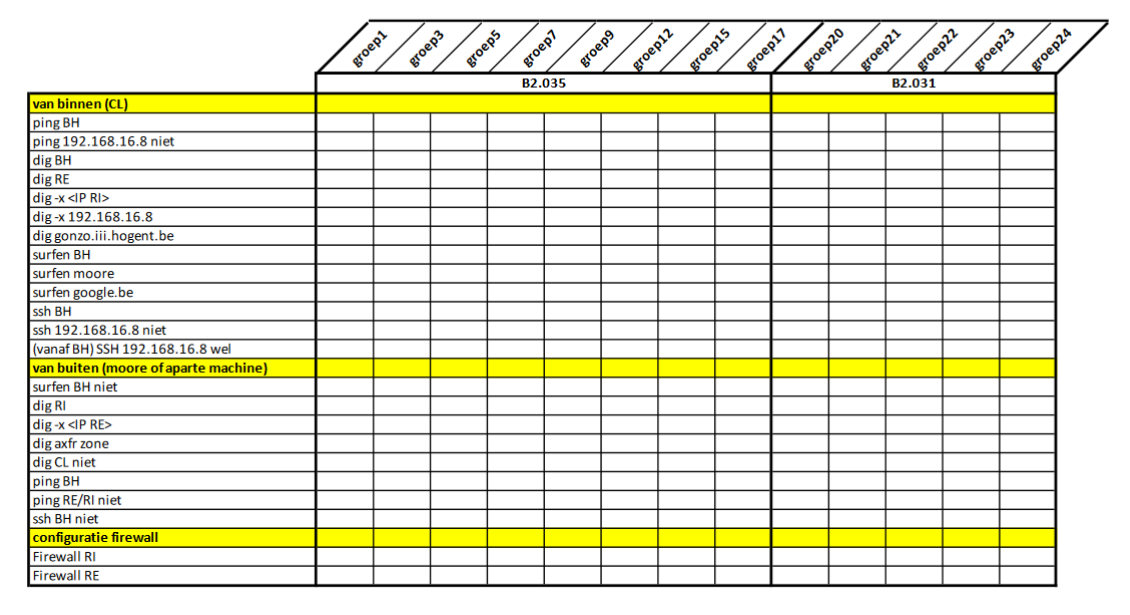
\includegraphics[width=\textwidth]{9_checklist}
	\caption{De checklist.}
	\label{fig:checklist}
\end{figure}

\section{Algemene richtlijnen}


Om deze opstelling te verwezenlijken moet de bestaande netwerkbekabeling worden aangepast.
Bedenk dat op het einde van de labosessie de oorspronkelijke toestand moet hersteld worden in een \textbf{werkende} staat.
Bij groepen die dit verzuimen zal de quotering worden aangepast!
Noteer dus alles goed vooraleer je iets verandert en test of de teruggeplaatste instellingen functioneren.

Bovendien moet je er rekening mee houden dat van elk paar UTP-netwerkcontactdozen op de tafel er steeds maar één connector is verbonden; onthoud dus de welke.
Ook is het van belang om van de twee (of meer) netwerkinterfaces in de pc's opnieuw de juiste te verbinden!

Bedenk ook dat eens het netwerk is onderbroken, het publieke internet en dus ook Minerva (tijdelijk) niet meer van op elke machine bereikbaar zijn.
Enkel de \textbf{externe router} blijft aangesloten op het "internet" met zijn origineel IP-adres. 







\end{document}

